%!TEX program = luatex

\documentclass[12pt]{article}
\usepackage[margin=0.8in]{geometry}
\usepackage{fontawesome}
\usepackage{fontspec}
\usepackage[hidelinks]{hyperref}
\usepackage{pdfpages}
\usepackage{csquotes}
\MakeOuterQuote{"}
\setmainfont{Palatino Linotype}
\setsansfont{Myriad Pro}
\setmonofont{Andale Mono}
\usepackage{microtype}

\usepackage{graphicx}
\setkeys{Gin}{width=\linewidth,totalheight=\textheight,keepaspectratio}
\graphicspath{{word365-img/}}


\setlength{\parindent}{0em}
\setlength{\parskip}{12pt}

\definecolor{fsuMaroon}{RGB}{155,0,33}
\definecolor{googleBlue}{RGB}{68,134,248}
\definecolor{googleBlue2}{RGB}{53,122,232}
\definecolor{sbGray}{HTML}{F6F6FF}
\definecolor{googleRed}{HTML}{D0402F}
\definecolor{darkgray}{rgb}{0.33, 0.33, 0.33}
\definecolor{amber}{rgb}{1.0, 0.49, 0.0}

\newcommand{\dueDate}[1]{\textbf{\textcolor{fsuMaroon}{#1}}}

\newcommand{\stepNo}[1]{\noindent\hangindent2em\textit{Step~#1.}}

\newcommand{\figImg}[1]{\begin{center}\frame{\includegraphics[width=0.75\linewidth]{#1.png}}\end{center}}

\newcommand{\buttonText}[1]{\fcolorbox{black}{amber}{\color{white}\textsf{\textbf{#1}}}}

\newcommand{\buttonTextRed}[1]{\fcolorbox{googleRed}{googleRed}{\color{white}\textsf{\textbf{\uppercase{#1}}}}}

\newcommand{\tabText}[1]{\fcolorbox{gray}{sbGray}{\color{black}\textsf{#1}}}

\newcommand{\linkText}[1]{\textcolor{darkgray}{\textsf{\textbf{#1}}}}

\newcommand{\keyText}[1]{\textsf{\faKeyboard~#1}}

\begin{document}

\begin{center}
\noindent\large\dueDate{\faBook}~~\textsf{\textit{Reference Sheet:} Word 365}\normalsize\\
\rule{4in}{1pt}
\end{center}

This reference sheet will lead you through the process of creating a document on Microsoft Word 365 (included in your tuition) and submitting it to TaskStream. Word 365 provides collaboration features that are not available through the "regular" offline Microsoft Word. In addition, the West Virginia Department of Education provides Microsoft Office 365 to all school districts in the state, so it is important to be familiar with it.

\stepNo{1} Log in to your Fairmont State web mail account and click on the "apps" button that looks like a nine-dot matrix. From the options that appear, select \linkText{Word Online}.
\figImg{1}

\stepNo{2} Word 365 will load in a new tab or window. When it is finished, it will provide you with a number of different templates to choose from. For this class, the \linkText{New blank document} template is OK. \linkText{APA-style paper} is available but is overkill for this course.
\begin{center}\frame{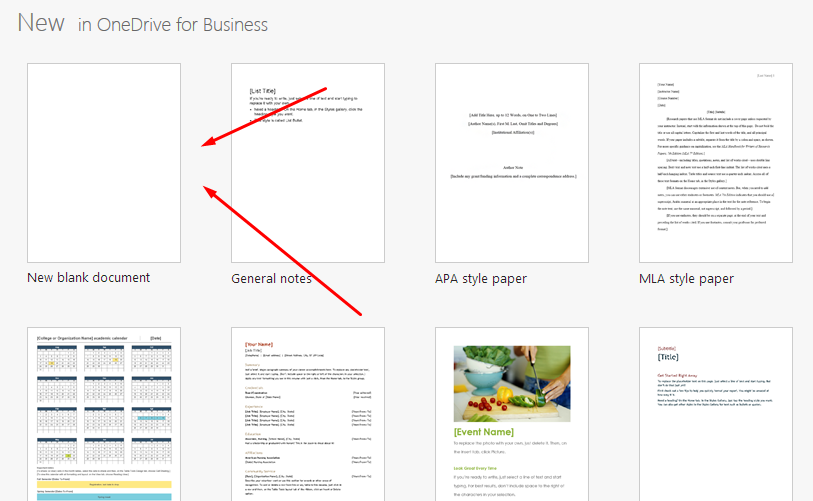
\includegraphics[width=0.5\linewidth]{2.png}}\end{center}

\newpage

\stepNo{3} You will now see a page that looks just like the "regular" offline Microsoft Word.
\figImg{3}

\stepNo{4} Now you may type and edit just like you do in the "regular" offline Microsoft Word. Note that your document is saved as you work.
\figImg{4}

\stepNo{5} When you are finished and fully satisfied with your work (and have edited it), click on the \buttonText{Share} button in the upper right corner of the screen.
\begin{center}\frame{
\includegraphics[width=0.35\linewidth]{5.png}}\end{center}

\newpage

\stepNo{6} The Share box will appear on the screen. First click on \linkText{Get Link} on the left-hand side and then click on \linkText{CREATE LINK} \textbf{UNDER THE EDIT HEADING}. Providing me a link without permission to edit (leave comments) will be returned.
\figImg{6}

\stepNo{7} Highlight the link address and then copy it by pressing \keyText{[Ctrl]-[C]}, \keyText{[Cmd]-[C]}, or right-click and click "Copy" from the menu to copy the link to your clipboard.
\figImg{7}

\newpage

\stepNo{8} Log into TaskStream and enter the course. Find the assignment that reads "Argument Paper" and click on it.
\begin{center}\frame{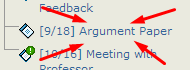
\includegraphics[width=0.35\linewidth]{8.png}}\end{center}

\stepNo{9} Click on the \buttonText{Links} button at the bottom of the screen to add your link.
\figImg{9}

\stepNo{10} Name your link as something like "Argument Essay" (1) and paste the link into the "Website URL" box (2). Then you may click on \buttonText{Add Link} (3).
\begin{center}\frame{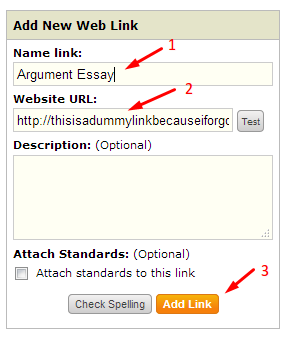
\includegraphics[width=0.35\linewidth]{10.png}}\end{center}

\stepNo{11} The screen will refresh. Click on \buttonText{Save and Return}.
\figImg{11}

\stepNo{12} Remember to take the next step and click on \buttonText{Submit Work}.
\figImg{12}

\stepNo{13} Lastly, let TaskStream know you really mean it and click on \buttonText{Yes - Submit My Work}. And that's it!
\figImg{13}

\end{document}
